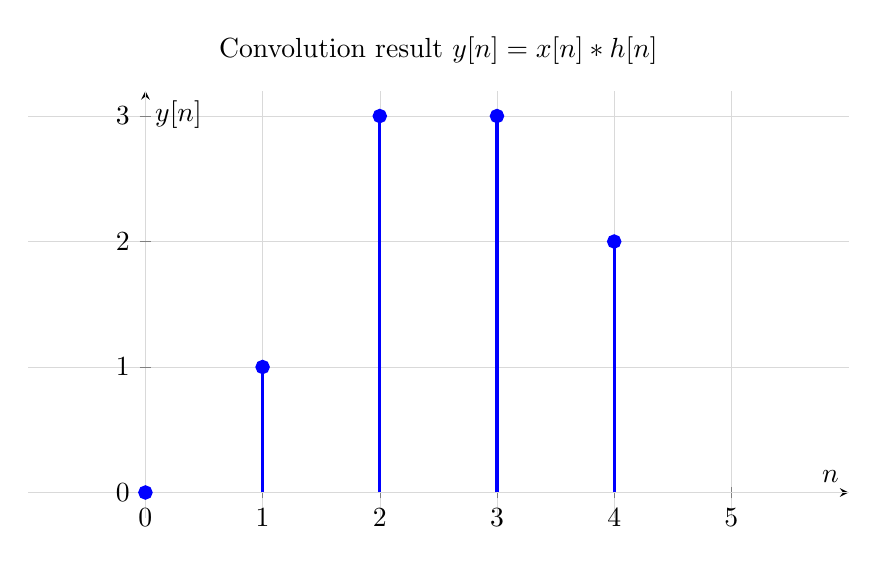
\begin{tikzpicture}
\begin{axis}[
    width=12cm,
    height=7cm,
    axis lines=middle,
    xlabel={$n$},
    ylabel={$y[n]$},
    title={Convolution result $y[n] = x[n] * h[n]$},
    xmin=-1, xmax=6,
    ymin=-0.2, ymax=3.2,
    xtick=\empty,
    ytick=\empty,
    extra x ticks={0, 1, 2, 3, 4, 5},
    extra y ticks={0, 1, 2, 3},
    grid=major,
    grid style={line width=.1pt, draw=gray!30},
]

% Plot the convolution result
\addplot[ycomb, blue, very thick, mark=*, mark size=2pt] coordinates {(0,0) (1,1) (2,3) (3,3) (4,2)};

\end{axis}
\end{tikzpicture}

